\documentclass[tikz,border=5pt]{standalone}
\usepackage[T1]{fontenc}
\usepackage{lmodern}
\usepackage{xcolor}
\usetikzlibrary{arrows.meta,calc,fit,positioning}

\definecolor{ink}{HTML}{17233B}
\definecolor{blue}{HTML}{2F6FED}
\definecolor{bluefill}{HTML}{EAF1FF}
\definecolor{teal}{HTML}{157A75}
\definecolor{tealfill}{HTML}{E8F6F4}
\definecolor{gold}{HTML}{A56B00}
\definecolor{goldfill}{HTML}{FFF5D8}
\definecolor{grayfill}{HTML}{F2F4F8}

\begin{document}
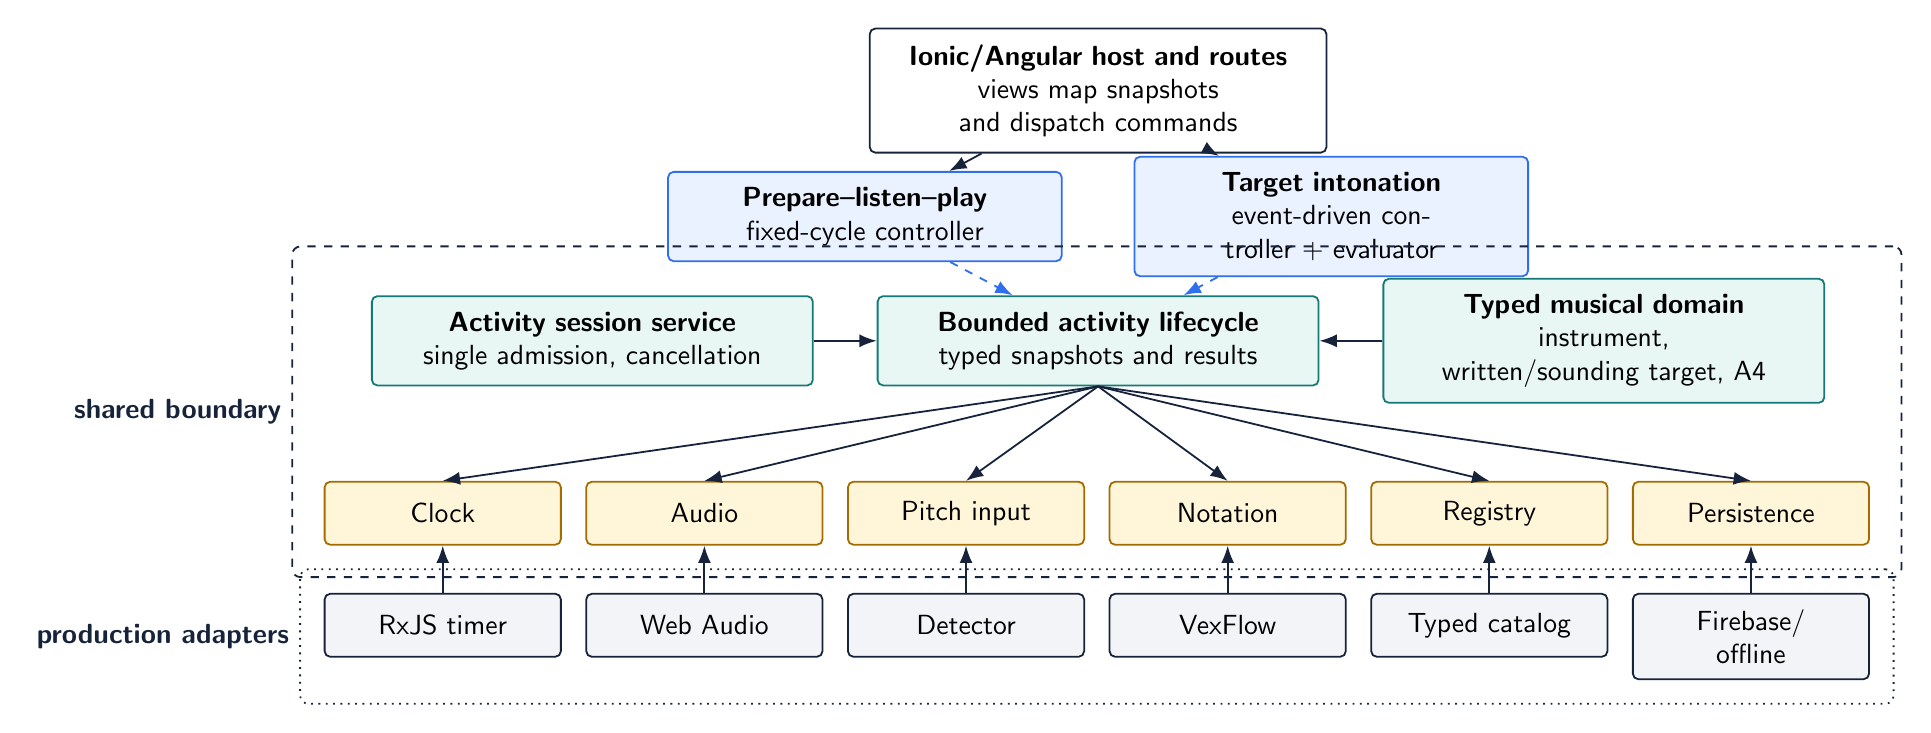
\begin{tikzpicture}[
  font=\sffamily,
  line width=.65pt,
  >={Latex[length=2.2mm]},
  box/.style={draw=ink, rounded corners=2pt, align=center,
    minimum height=9mm, inner xsep=4mm, inner ysep=2mm},
  activity/.style={box, draw=blue, fill=bluefill, text width=42mm},
  shared/.style={box, draw=teal, fill=tealfill, text width=48mm},
  port/.style={box, draw=gold, fill=goldfill, text width=22mm,
    minimum height=8mm},
  adapter/.style={box, fill=grayfill, text width=22mm, minimum height=8mm},
  flow/.style={->, draw=ink},
  depends/.style={->, draw=blue, dashed}
]

\node[activity] (plp) {\textbf{Prepare--listen--play}\\fixed-cycle controller};
\node[activity, right=9mm of plp] (intonation)
  {\textbf{Target intonation}\\event-driven controller + evaluator};

\node[shared, below=10mm of $(plp)!0.5!(intonation)$] (lifecycle)
  {\textbf{Bounded activity lifecycle}\\typed snapshots and results};
\node[shared, left=8mm of lifecycle] (session)
  {\textbf{Activity session service}\\single admission, cancellation};
\node[shared, right=8mm of lifecycle] (domain)
  {\textbf{Typed musical domain}\\instrument,\\written/sounding target, A4};

\node[port, below=12mm of session, xshift=-19mm] (clock) {Clock};
\node[port, right=3mm of clock] (audio) {Audio};
\node[port, right=3mm of audio] (pitch) {Pitch input};
\node[port, right=3mm of pitch] (notation) {Notation};
\node[port, right=3mm of notation] (registry) {Registry};
\node[port, right=3mm of registry] (persist) {Persistence};

\node[adapter, below=6mm of clock] (clocka) {RxJS timer};
\node[adapter, below=6mm of audio] (audioa) {Web Audio};
\node[adapter, below=6mm of pitch] (pitcha) {Detector};
\node[adapter, below=6mm of notation] (notationa) {VexFlow};
\node[adapter, below=6mm of registry] (registrya) {Typed catalog};
\node[adapter, below=6mm of persist] (persista) {Firebase/\\offline};

\node[box, fill=white, text width=50mm, above=8mm of $(plp)!0.5!(intonation)$]
  (host) {\textbf{Ionic/Angular host and routes}\\views map snapshots and dispatch commands};

\draw[flow] (host) -- (plp);
\draw[flow] (host) -- (intonation);
\draw[depends] (plp) -- (lifecycle);
\draw[depends] (intonation) -- (lifecycle);
\draw[flow] (session) -- (lifecycle);
\draw[flow] (domain) -- (lifecycle);

\foreach \p in {clock,audio,pitch,notation,registry,persist}
  \draw[flow] (lifecycle.south) -- (\p.north);
\foreach \p/\a in {clock/clocka,audio/audioa,pitch/pitcha,notation/notationa,
                   registry/registrya,persist/persista}
  \draw[flow] (\a) -- (\p);

\node[draw=ink, dashed, rounded corners=3pt, fit=(session)(lifecycle)(domain)
      (clock)(persist), inner sep=4mm,
      label={[font=\sffamily\bfseries, text=ink]left:shared boundary}] {};
\node[draw=ink, dotted, rounded corners=3pt,
      fit=(clocka)(persista), inner sep=3mm,
      label={[font=\sffamily\bfseries, text=ink]left:production adapters}] {};

\end{tikzpicture}
\end{document}
